\documentclass[tikz,border=6pt]{standalone}
\usepackage{amsmath}
\usepackage{newtxtext,newtxmath}
\usetikzlibrary{arrows.meta,calc}

\begin{document}
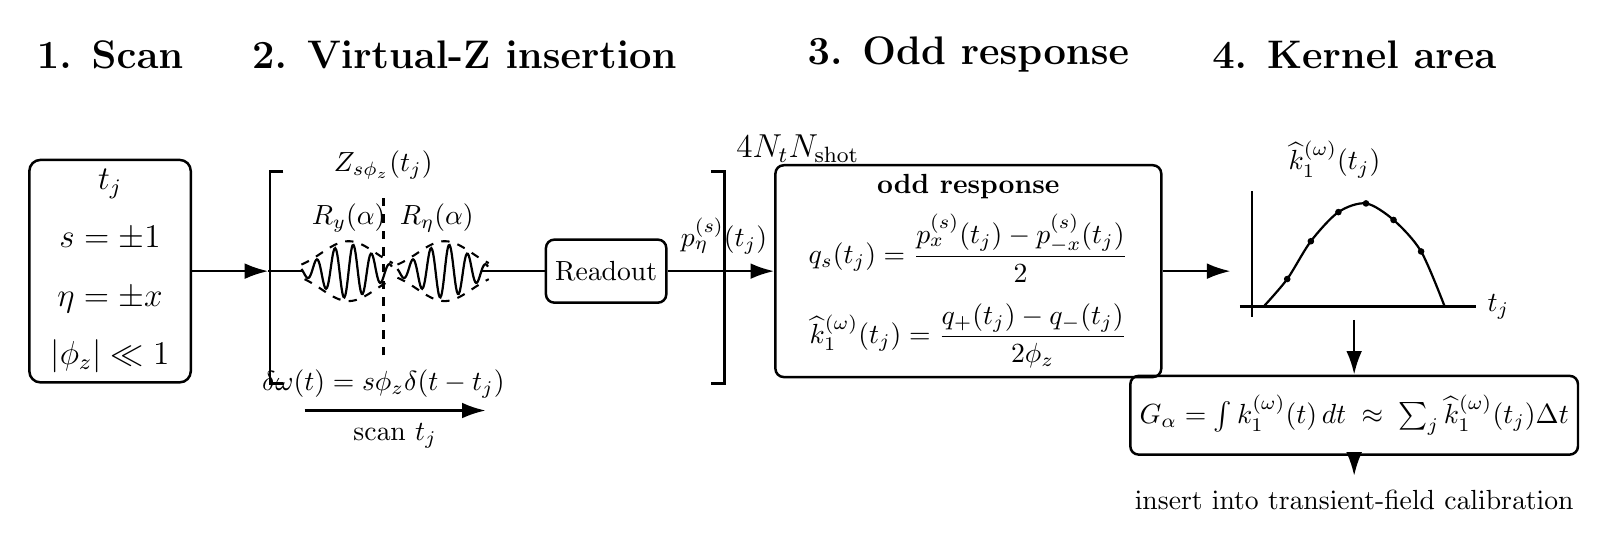
\begin{tikzpicture}[
  x=1cm,
  y=1cm,
  >=Latex,
  font=\large,
  line/.style={draw=black,line width=0.9pt},
  arrow/.style={line,-{Latex[length=3mm,width=2mm]}},
  block/.style={line,rounded corners=3pt,align=center,minimum height=0.8cm},
  smallblock/.style={block,minimum width=1.3cm,font=\normalsize},
  extractbox/.style={line,rounded corners=3pt,align=center,minimum width=4.9cm,minimum height=2.5cm,font=\normalsize},
  setbox/.style={line,rounded corners=4pt,align=center,minimum width=2.05cm,minimum height=2.55cm},
  pulse/.style={line,line width=0.8pt},
  envelope/.style={line,dashed,line width=0.75pt}
]

% Section headings
\node[font=\bfseries\Large] at (1.25,3.10) {1. Scan};
\node[font=\bfseries\Large] at (5.75,3.10) {2. Virtual-Z insertion};
\node[font=\bfseries\Large] at (12.15,3.10) {3. Odd response};
\node[font=\bfseries\Large] at (17.05,3.10) {4. Kernel area};

% Scan parameters
\node[setbox] (scan) at (1.25,0.35)
  {$t_j$\\[0.25cm]$s=\pm1$\\[0.25cm]$\eta=\pm x$\\[0.25cm]$|\phi_z|\ll1$};

% Measurement bracket
\draw[line width=1pt]
  (3.45,1.62) -- (3.28,1.62) -- (3.28,-1.08) -- (3.45,-1.08);
\draw[line width=1pt]
  (8.88,1.62) -- (9.05,1.62) -- (9.05,-1.08) -- (8.88,-1.08);
\node[anchor=south west,font=\large] at (9.08,1.60) {$4N_tN_{\mathrm{shot}}$};

\draw[arrow] (scan.east) -- (3.26,0.35);
\draw[line] (3.26,0.35) -- (3.7,0.35);

% Pulse sequence, with adjacent Gaussian pulses
\node[font=\normalsize] at (4.28,1.02) {$R_y(\alpha)$};
\begin{scope}[shift={(4.28,0.35)}]
  \draw[pulse,domain=-0.6:0.55,samples=100,smooth]
    plot (\x,{0.34*exp(-5*\x*\x)*sin(deg(27*\x))});
  \draw[envelope,domain=-0.6:0.56,samples=60,smooth]
    plot (\x,{0.38*exp(-4.2*\x*\x)});
  \draw[envelope,domain=-0.56:0.56,samples=60,smooth]
    plot (\x,{-0.38*exp(-4.2*\x*\x)});
\end{scope}

\node[font=\normalsize] at (5.40,1.02) {$R_{\eta}(\alpha)$};
\begin{scope}[shift={(5.5,0.35)}]
  \draw[pulse,domain=-0.6:0.55,samples=100,smooth]
    plot (\x,{0.34*exp(-5*\x*\x)*sin(deg(27*\x))});
  \draw[envelope,domain=-0.6:0.56,samples=60,smooth]
    plot (\x,{0.38*exp(-4.2*\x*\x)});
  \draw[envelope,domain=-0.6:0.56,samples=60,smooth]
    plot (\x,{-0.38*exp(-4.2*\x*\x)});
\end{scope}

% Virtual-Z insertion at one scanned time
\draw[line,dashed] (4.72,-0.72) -- (4.72,1.36);
\node[font=\normalsize,anchor=south] at (4.72,1.39) {$Z_{s\phi_z}(t_j)$};
\node[font=\normalsize,anchor=north] at (4.72,-0.78)
  {$\delta\omega(t)=s\phi_z\delta(t-t_j)$};

% Scan direction marker
\draw[arrow] (3.72,-1.42) -- (6.02,-1.42);
\node[font=\normalsize,anchor=north] at (4.87,-1.46) {scan $t_j$};

\node[smallblock,minimum width=1.1cm] (readout) at (7.55,0.35) {Readout};
\draw[line] (5.96,0.35) -- (readout.west);

% Differential extraction
\node[extractbox] (extract) at (12.15,0.35)
  {\textbf{odd response}\\[0.16cm]
   $q_s(t_j)=\dfrac{p_x^{(s)}(t_j)-p_{-x}^{(s)}(t_j)}{2}$\\[0.24cm]
   $\widehat{k}_1^{(\omega)}(t_j)=
   \dfrac{q_{+}(t_j)-q_{-}(t_j)}{2\phi_z}$};
\draw[arrow] (readout.east) -- node[above,font=\normalsize,pos=0.53,yshift=0.08cm]
  {$p_{\eta}^{(s)}(t_j)$} (extract.west);

% Kernel plot and area
\begin{scope}[shift={(17.05,0.55)}]
  \draw[line] (-1.45,-0.65) -- (1.55,-0.65);
  \draw[line] (-1.30,-0.78) -- (-1.30,0.82);
  \draw[pulse,smooth]
    plot coordinates {(-1.15,-0.65) (-0.85,-0.30) (-0.55,0.18) (-0.20,0.55)
      (0.15,0.66) (0.50,0.45) (0.85,0.05) (1.15,-0.65)};
  \fill (-0.85,-0.30) circle (1.2pt);
  \fill (-0.55,0.18) circle (1.2pt);
  \fill (-0.20,0.55) circle (1.2pt);
  \fill (0.15,0.66) circle (1.2pt);
  \fill (0.50,0.45) circle (1.2pt);
  \fill (0.85,0.05) circle (1.2pt);
  \node[font=\normalsize,anchor=west] at (1.57,-0.65) {$t_j$};
  \node[font=\normalsize,anchor=south] at (-0.25,0.86)
    {$\widehat{k}_1^{(\omega)}(t_j)$};
\end{scope}

\node[block,minimum width=4.15cm,minimum height=1.0cm,font=\normalsize] (area) at (17.05,-1.48)
  {$G_\alpha=\int k_1^{(\omega)}(t)\,dt
   \;\approx\;\sum_j\widehat{k}_1^{(\omega)}(t_j)\Delta t$};
\draw[arrow] (extract.east) -- (15.48,0.35);
\draw[arrow] (17.05,-0.27) -- (area.north);

\node[font=\normalsize,align=center] at (17.05,-2.55)
  {insert into transient-field calibration};
\draw[arrow] (area.south) -- (17.05,-2.25);

\end{tikzpicture}
\end{document}
